\chapter{Anti-Aliasing Filter Considerations} \label{App:AntiAliasingFilterConsideration}

A number of filter types were evaluated to see their frequency responses. The MATLAB code for this can be seen in listng \refq{lst:A_AA_FILTER_CODE}.
\lstinputlisting[language=C ,style = c,firstnumber=1, linerange=1-81, caption={MATLAB code for evaluating filter types.}, label={lst:A_AA_FILTER_CODE}]{Appendix/code/AntiAliasingFiltre.m}. 

The magnitude response for the different filter types can be seen on figure \refq{fig:A_FILT_MAG}.

\begin{figure}[H]
    \centering
    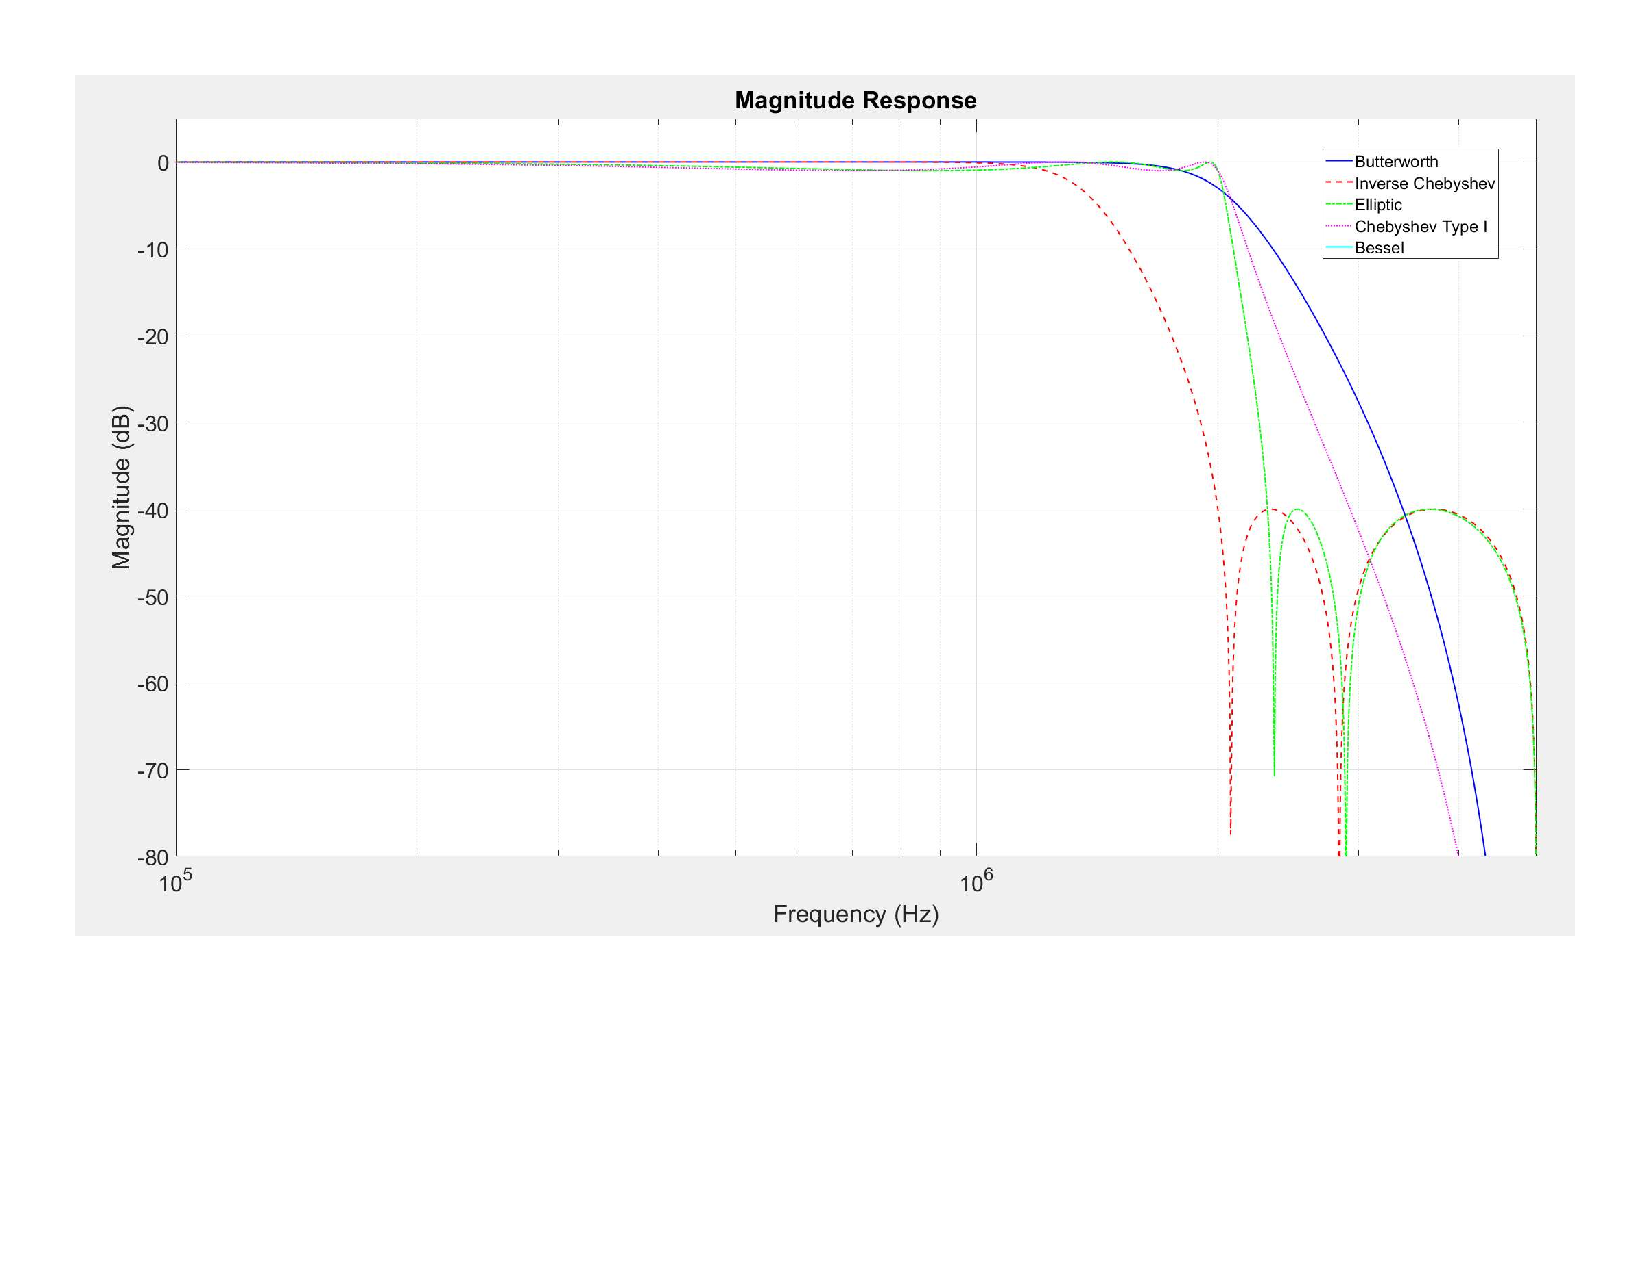
\includegraphics[clip, trim=0 150 0 0, width=1\textwidth]{Appendix/Figures/A_FILT_MAG.pdf}
    \caption{Magnitude response of various filter types.}
    \label{fig:A_FILT_MAG}
\end{figure}

The phase response can be seen on figure \refq{fig:A_FILT_PHASE}.

\begin{figure}[H]
    \centering
    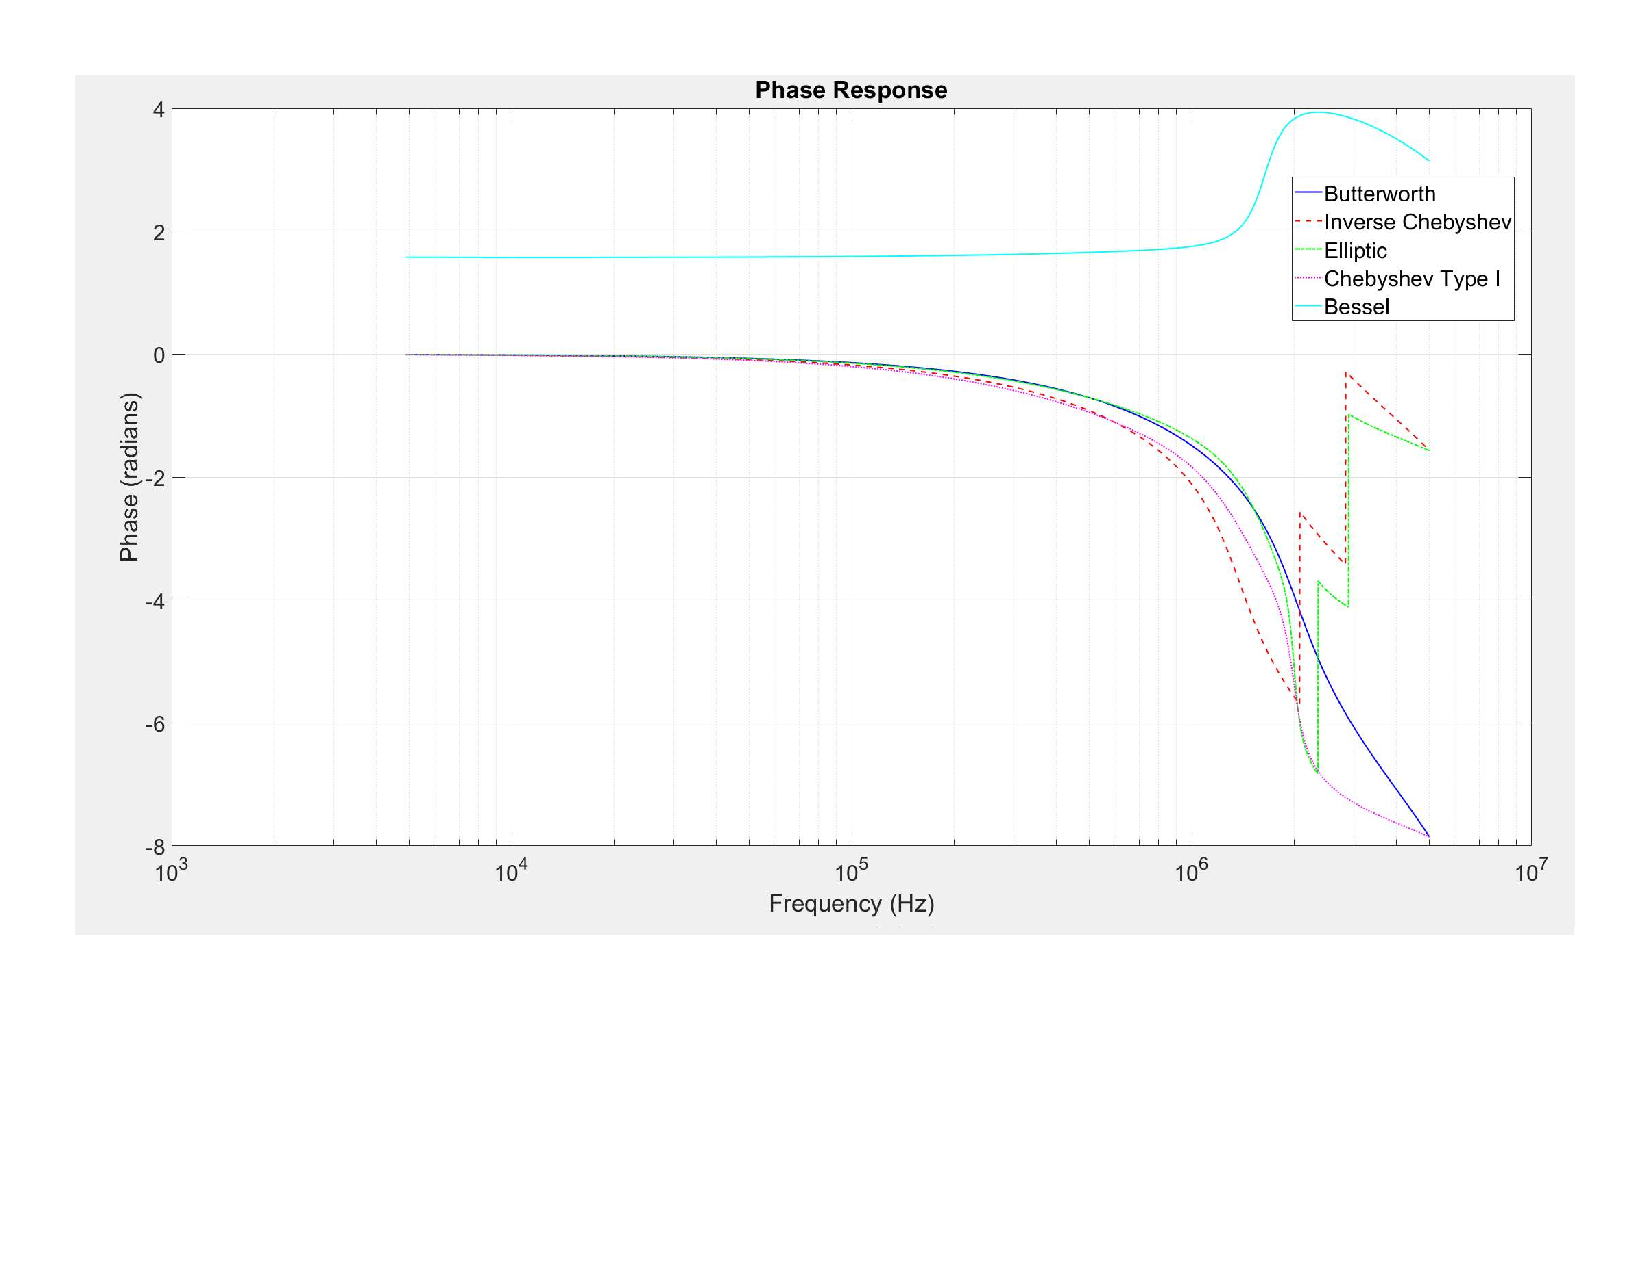
\includegraphics[clip, trim=0 150 0 0, width=1\textwidth]{Appendix/Figures/A_FILT_PHASE.pdf}
    \caption{Phase response of various filter types.}
    \label{fig:A_FILT_PHASE}
\end{figure}

The group delay response can be seen on figure \refq{fig:A_FILT_GROUP}.

\begin{figure}[H]
    \centering
    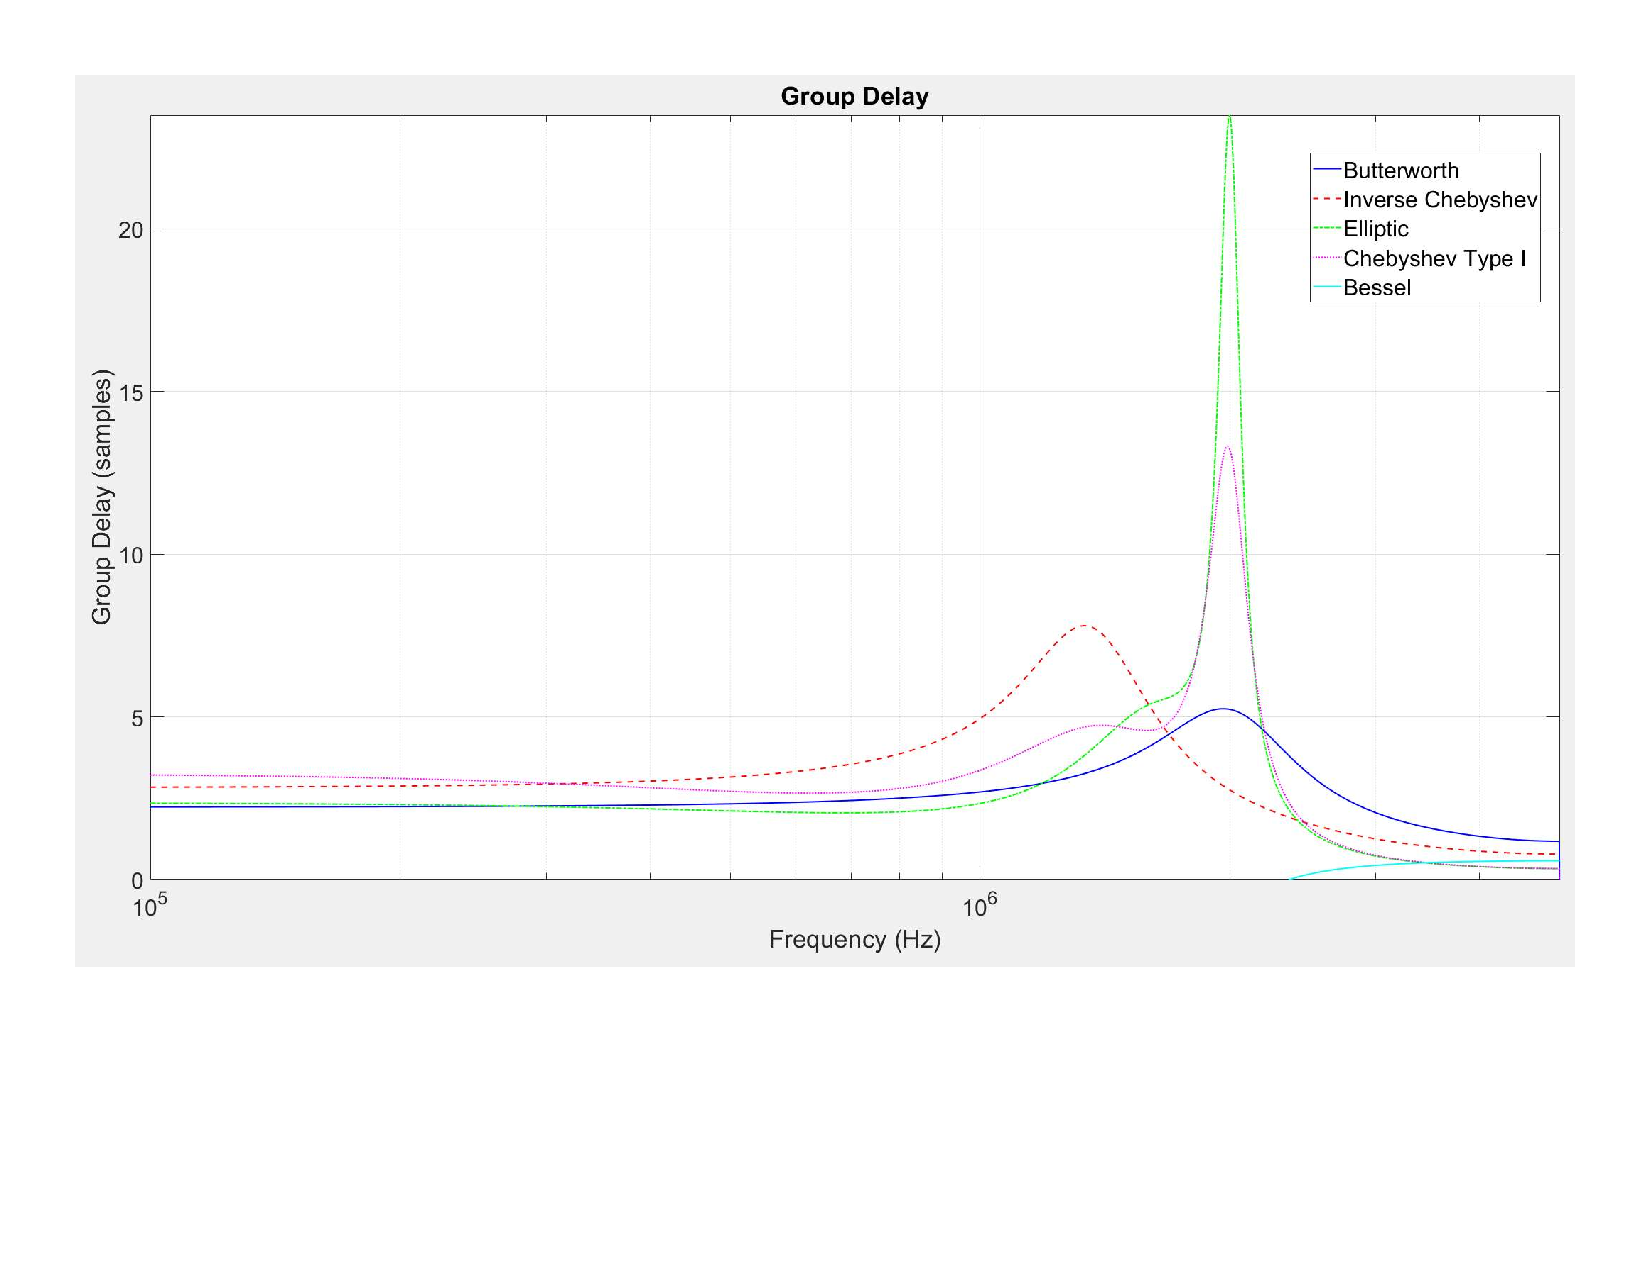
\includegraphics[clip, trim=0 150 0 0, width=1\textwidth]{Appendix/Figures/A_FILT_GROUP.pdf}
    \caption{Group delay for the various filter types.}
    \label{fig:A_FILT_GROUP}
\end{figure}

The Anti-Aliasing filter should have maximum passband flatness, so based on figure \refq{fig:A_FILT_MAG} butterworth, bessel and inverse chebychev lowpass filters could be used. The filter will be a butterworth filter based on this.

To see the effects of varying the order of a butterworth filter, the MATLAB code in listing \refq{lst:A_AA_BUT_CUDE} was used.

\lstinputlisting[language=C ,style = c,firstnumber=1, linerange=1-44, caption={MATLAB code for evaluating the order of a butterworth filter}, label={lst:A_AA_BUT_CUDE}]{Appendix/Code/AntiAliasingFilterOrder.m}. 

The magnitude responses of the butterworth filters can be seen on figure \refq{fig:A_FILT_MAG_BUT}
\begin{figure}[H]
    \centering
    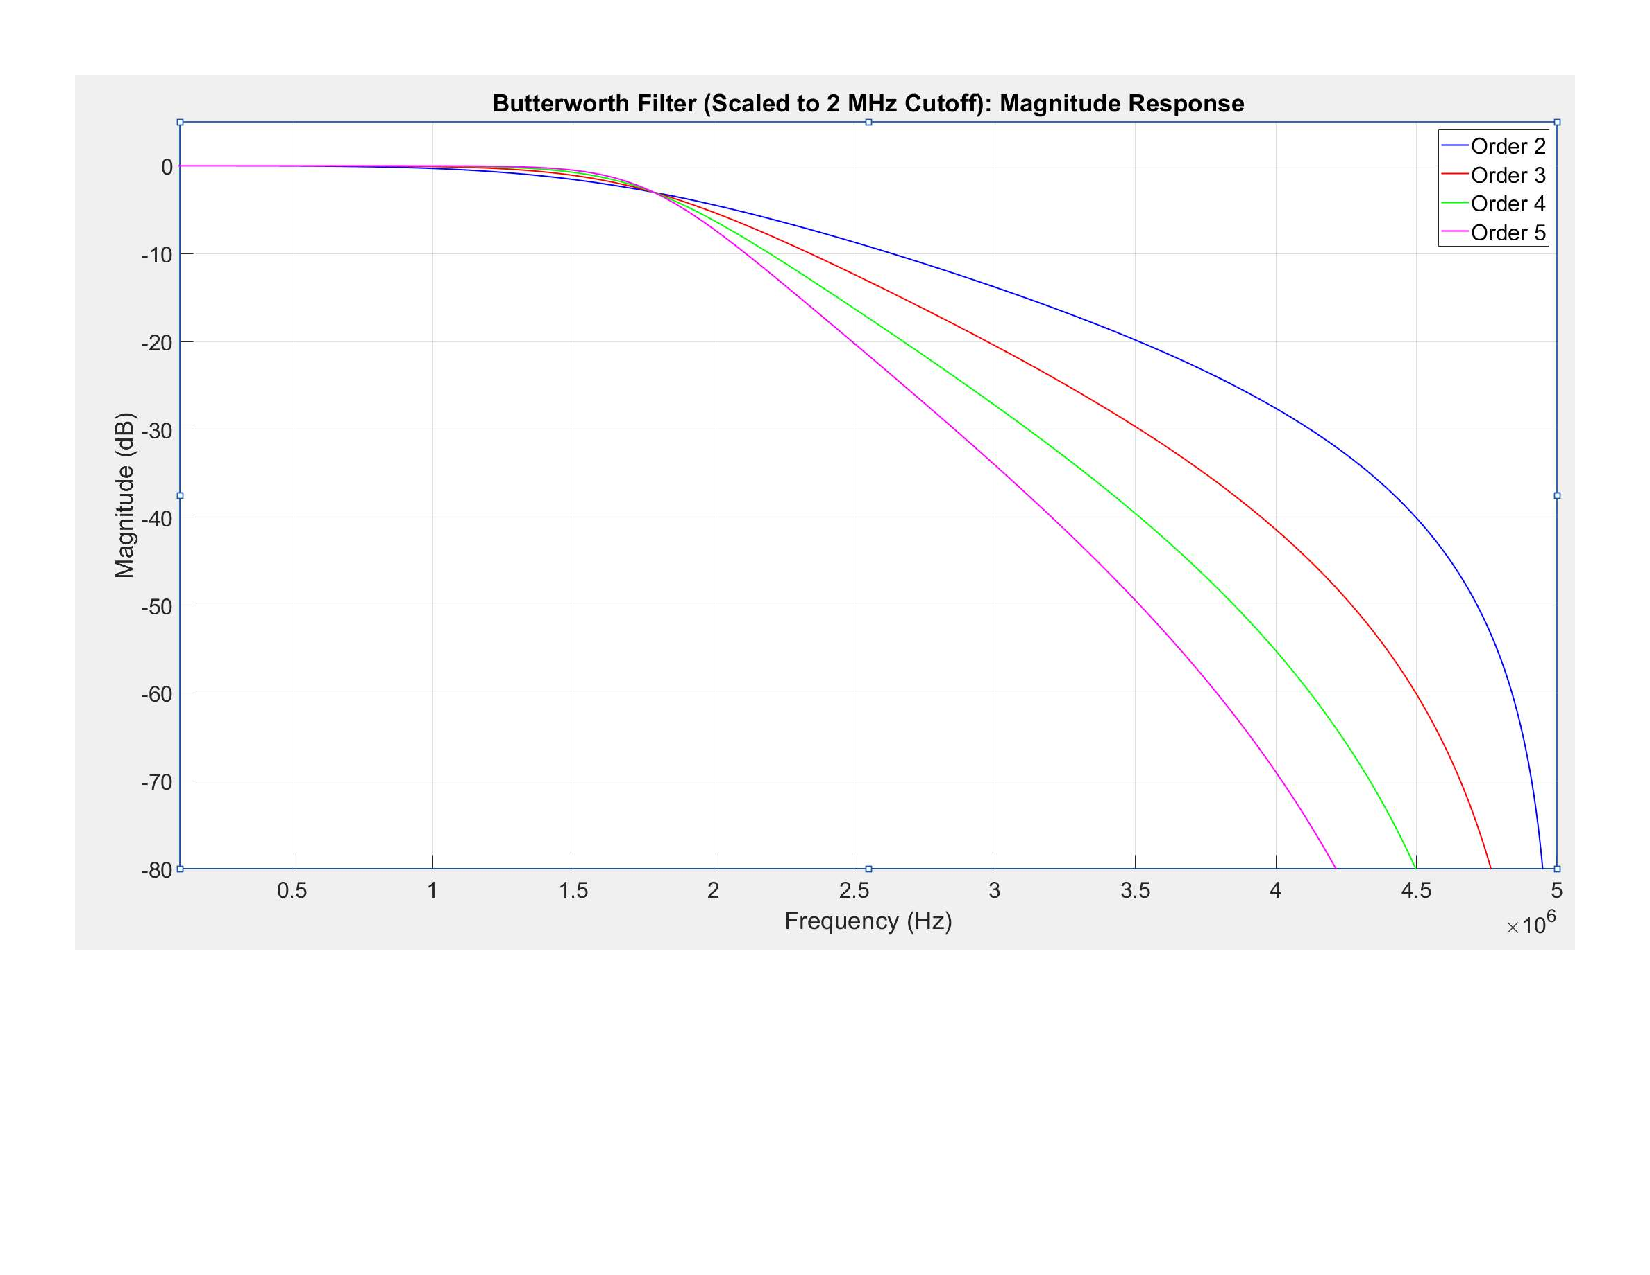
\includegraphics[clip, trim=0 150 0 0, width=1\textwidth]{Appendix/Figures/A_FILT_BUT_MAG.pdf}
    \caption{Magnitude plots for n=2, n=3, n=4, n=5 orders of a butterworth filter with a cut-off frequency at 2MHz.}
    \label{fig:A_FILT_MAG_BUT}
\end{figure}

The highest test signal frequency in the system is expected to be 1MHz. The gain at this frequency is of particular interest, there should be little change in ampltitude under 1MHz. The code in listing \refq{lst:A_AA_BUT_COMP} was used to compared the difference at 1MHz.

\lstinputlisting[language=C ,style = c,firstnumber=1, linerange=1-44, caption={MATLAB code for comparing the gain at 1MHz for different orders of a butterworth filter.}, label={lst:A_AA_BUT_COMP}]{Appendix/Code/AntiAliasingFilterComparison.m}. 

The results for the comparison can be seen on figure \refq{fig:A_FILT_MAG_COMP}.

\begin{figure}[H]
    \centering
    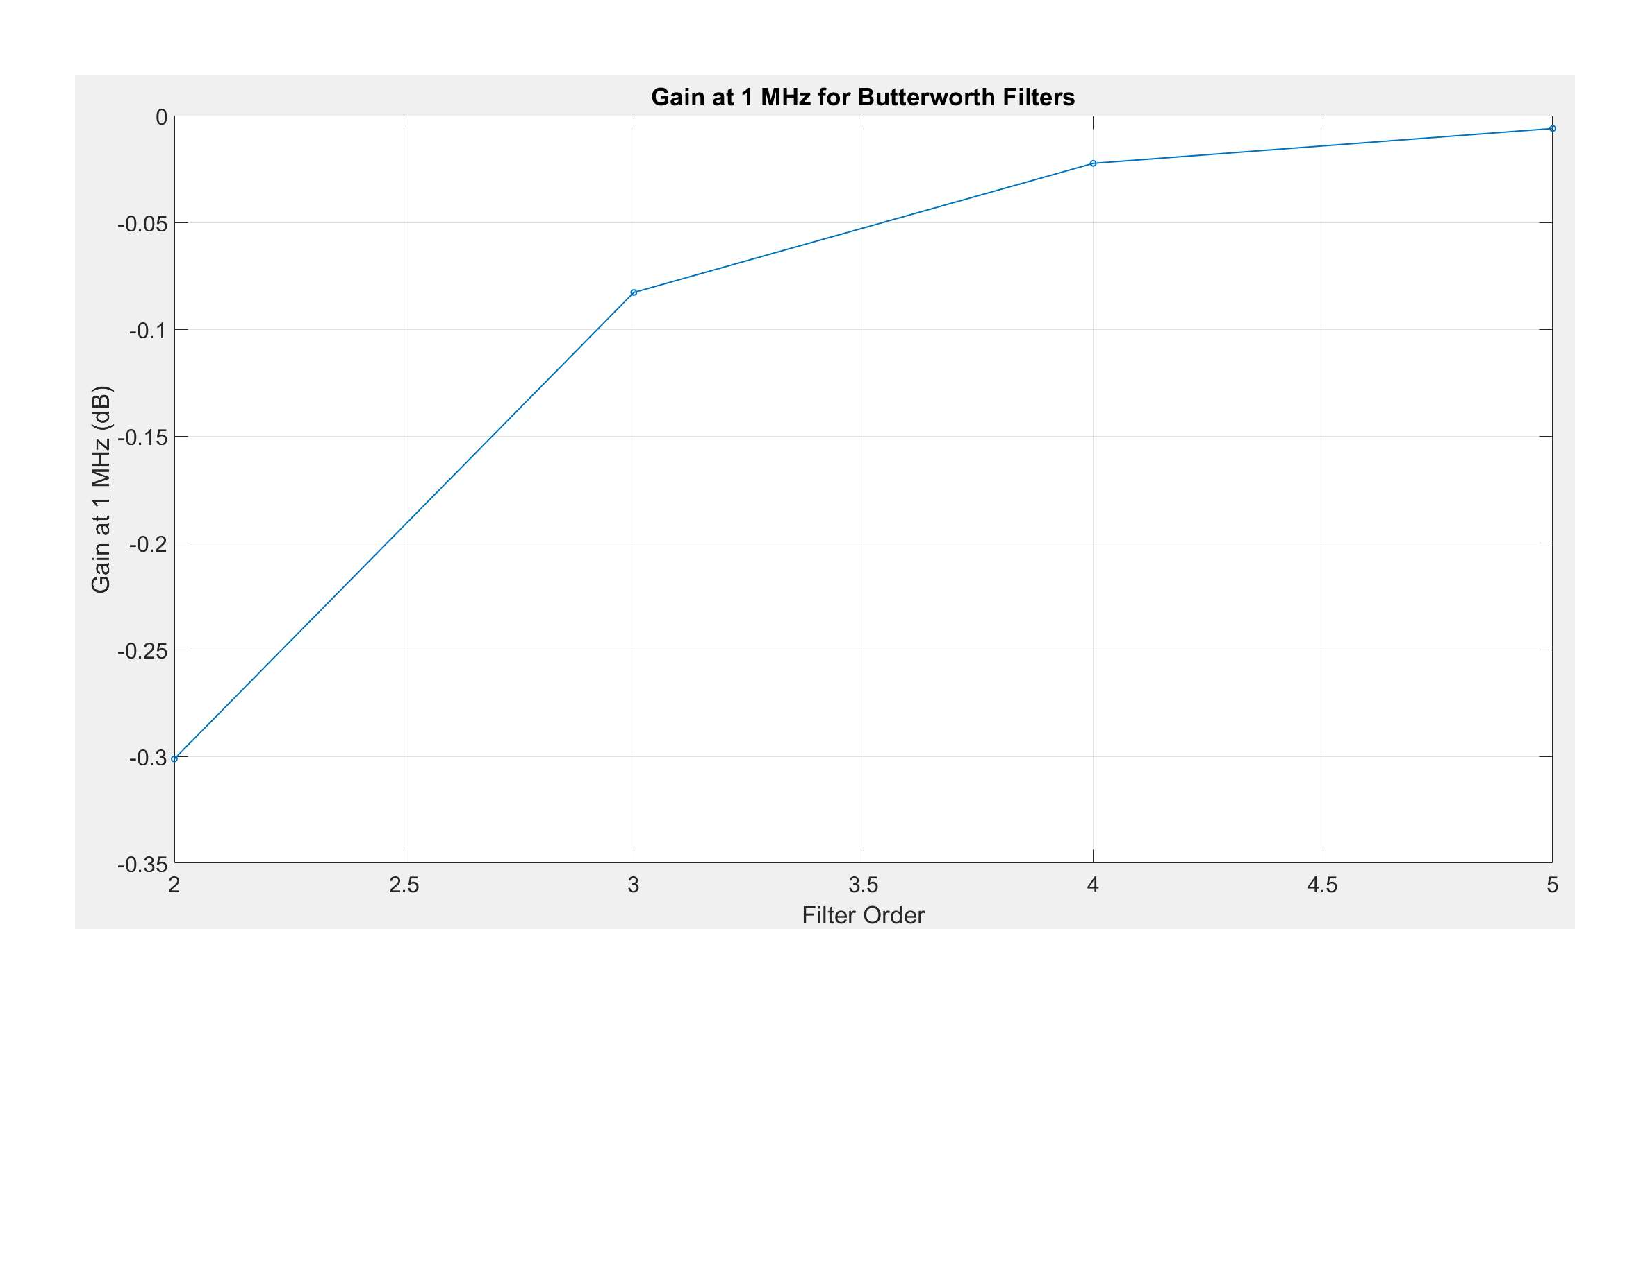
\includegraphics[clip, trim=0 150 0 0, width=1\textwidth]{Appendix/Figures/A_FILT_BUT_COMP.pdf}
    \caption{Comparing the difference in gain at 1MHz for a butterworth of n=2, n=3, n=4, n=5 orders.}
    \label{fig:A_FILT_MAG_COMP}
\end{figure}

A butterworth with a cut-off at \SIQ{2}{\mega\hertz} will attenuate \SIQ{1}{\mega\hertz} frequencies with \SIQ{-0.3}{\decibel}. Doubling the number of order to $n = 4$ brings the attenuation at \SIQ{1}{\mega\hertz} down to less than \SIQ{-0.05}{\decibel} while increasing it up to $n = 5$ is only a marginal change from $n = 4$. Based on this the anti-alising filter will be a 4th order butterworth filter.  